\documentclass[runningheads]{llncs}
\usepackage[T1]{fontenc}

\usepackage{tikz}
\usepackage{graphicx}
\usepackage{listings}
\usepackage{hyperref}
\usetikzlibrary{patterns}

% Definizione dei colori per la sintassi
\definecolor{everforestBg}{HTML}{fffbef}
\definecolor{everforestFg}{HTML}{5c6a72}
\definecolor{everforestRed}{HTML}{f85552}
\definecolor{everforestGreen}{HTML}{8da101}
\definecolor{everforestYellow}{HTML}{dfa000}
\definecolor{everforestBlue}{HTML}{3a94c5}
\definecolor{everforestPurple}{HTML}{df69ba}
\definecolor{everforestAqua}{HTML}{35a77c}
\definecolor{everforestOrange}{HTML}{f57d26}
\definecolor{everforestGray}{HTML}{939f91}
\lstdefinelanguage{AgentSpeak}{
  alsoletter={.},
  keywords={
    true, false, not, &, |, if, else, for, while,
    go_to_clean, move_to, find_and_clean, gain, clean,
    .wait, .print, .my_name, .send
  },
  keywords=[2]{
    my_region, dirt, ntpp, cleaned, gained
  },
  keywords=[3]{
    Dirt, Region
  },
  sensitive=true,
  comment=[l]{//},
  morecomment=[s]{/*}{*/},
  morestring=[b]",
  morestring=[b]',
  moredelim=**[s][\color{everforestRed}]{!}{\ },
  moredelim=**[s][\color{everforestRed}]{+!}{\ },
  moredelim=**[s][\color{everforestRed}]{-!}{\ },
  moredelim=**[s][\color{everforestRed}]{?}{\ },
  moredelim=**[s][\color{everforestRed}]{+}{\ },
  moredelim=**[s][\color{everforestRed}]{-}{\ },
  moredelim=**[s][\color{everforestRed}]{<-}{\ },
  moredelim=**[s][\color{everforestRed}]{:}{\ },
  moredelim=**[s][\color{everforestRed}]{;}{\ },
}

%\lstdefinelanguage{AgentSpeak}{
%  alsoletter={., _},
%  keywords={dirt, my_region},
%  sensitive=true,
%  comment=[l]{//},
%  morecomment=[s]{/*}{*/},
%  morestring=[b]",
%  moredelim=**[s][\color{everforestRed}]{+!}{\ },
%  moredelim=**[s][\color{everforestRed}]{!}{\ },
%  moredelim=**[s][\color{everforestRed}]{-}{\ },
%  moredelim=**[s][\color{everforestRed}]{<-}{\ },
%  moredelim=**[s][\color{everforestRed}]{:}{\ },
%  moredelim=**[s][\color{everforestRed}]{&}{\ },
%  moredelim=**[s][\color{everforestAqua}]{.}{(},
%}

\lstset{
    keywordstyle=\color{everforestAqua}\bfseries,
    keywordstyle=[2]\color{everforestBlue},
    keywordstyle=[3]\color{everforestFg},
    keywordstyle=[4]\color{everforestRed},
    commentstyle=\color{gray}\itshape,
    stringstyle=\color{everforestYellow},
    basicstyle=\ttfamily\small,
    backgroundcolor=\color{white},
    rulecolor=\color{black},
    tabsize=2,
    captionpos=b,
    breaklines=true,
    breakatwhitespace=false,
    showspaces=false,
    showstringspaces=false,
    showtabs=false
}

%\lstset{
%  language=AgentSpeak,
%  backgroundcolor=\color{white},
%  basicstyle=\color{everforestFg}\ttfamily\small,
%  keywordstyle=\color{everforestAqua},
%  commentstyle=\color{everforestGreen},
%  stringstyle=\color{everforestOrange},
%  numberstyle=\color{everforestFg},
%  identifierstyle=\color{everforestFg},
%  breaklines=true,
%  breakatwhitespace=true,
%  showstringspaces=false,
%  columns=flexible,
%  keepspaces=true
%}

\title{Towards a Continous Cleaning Robot}
\author{Andrea Gatti\orcidID{0009-0003-0992-4058}}
\institute{University of Genoa \\ \email{\url{andrea.gatti@edu.unige.it}}}

\begin{document}
	\maketitle

	\begin{abstract}
    Cleaning vacuum cleaner robot is a common didactic example in the field of multi-agent systems.
    Normally, the robot is placed inside a grid world and reasons directly on the step to perform.
    In this work, we present a different approach where the robot is placed in a continuous environment and reasons in a more abstract way on regions instead of cells.
    In this way, the agent is able to abstract more and focus on high-level tasks instead of low-level details.

		\keywords{Intelligent Agents \and Virtual Environment \and Cleaning Robot.}
	\end{abstract}

	\section{Introduction and Motivation}
	\label{sec:introduction}
The cleaning robot is a classical problem in the Multi-Agent System literature.
Normally, the cleaning robot is a robot that moves in a grid environment and cleans the dirty cells.
The reasoning about the cleaning robot is usually done in a discrete way, where the robot moves from one cell to another.

	\section{Design and Implementation}
	\label{sec:design_and_implementation}
To implement an agent that reasons logically about regions and takes advantage of simulation software to do path finding, it is necessary to choose the most suitable tools.
Since there is no framework for implementing BDI agents on major game engines, it was necessary to separate the two components and create a connection between them.
The first component handles the intelligent agent and the second handles the physical body and environment. The framework must ensure a 1-to-1 connection between the BDI agent and its body.
The architecture can be seen in Figure\ref{fig:architecture}.

\begin{figure}
    \centering
    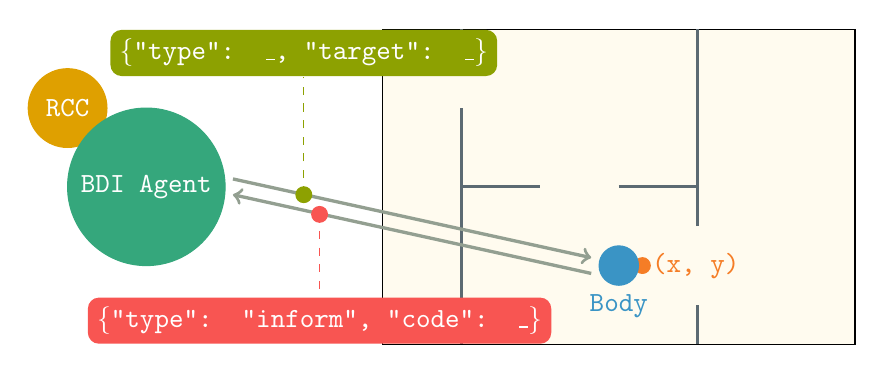
\begin{tikzpicture}
    \draw[fill=everforestYellow, everforestYellow] (-1, 1) circle (0.5cm) node[white]{\texttt{RCC}};
    \draw[fill=everforestAqua, everforestAqua] (0, 0) circle (1cm) node[white]{\texttt{BDI Agent}};
    \draw[fill=everforestBg] (3, -2) rectangle ++ (6, 4);
    \draw[very thick, everforestFg] (4, -2) -- (4, 1) (4, 0) -- (5, 0) (6, 0) -- (7, 0) (7, -0.5) -- (7, 2) (7, -2) -- (7, -1.5) (4, 1.5) -- (4, 2);
    \draw[fill=everforestOrange, everforestOrange] (6.3, -1) circle (0.1cm) node[right]{\texttt{(x, y)}};
    \draw[fill=everforestBlue, everforestBlue] (6, -1) circle (0.25cm) node[below=0.25cm]{\texttt{Body}};
    \draw[->, very thick, everforestGray] (1.1, 0.1) -- (5.65, -0.9);
    \draw[<-, very thick, everforestGray] (1.1, -0.1) -- (5.65, -1.1);

    \draw[fill=everforestGreen, everforestGreen] (2, -0.1) circle (0.1cm);
    \draw[everforestGreen, dashed] (2, -0.1) -- (2, 1.4) node[above, white, fill=everforestGreen, rounded corners]{\texttt{\{"type": \_, "target": \_\}}};

    \draw[fill=everforestRed, everforestRed] (2.2, -0.35) circle (0.1cm);
    \draw[everforestRed, dashed] (2.2, -0.35) -- (2.2, -1.4) node[below, white, fill=everforestRed, rounded corners]{\texttt{\{"type": "inform", "code": \_\}}};
\end{tikzpicture}
    \label{fig:architecture}
    \caption{The architecture of the system}
\end{figure}

The section is now divided into three subsections. The first lays some fundamentals to be shared by agent and environment on the Region Connection Calculus (RCC) and the environment in which the simulation will take place, the second presents the design and implementation of the BDI agent, and the third follows the same path for the virtual environment.

\subsection{Environment and Regions}
The environment and agent must properly implement the principles of Region Connection Calculus (RCC) introduced by D. A. Randell, Z. Cui and A. G. Cohn\cite{DBLP:conf/kr/RandellCC92}.
RCC provides some basic relationships between regions that are visible in Figure\ref{fig:relations}.
With these relationships it is possible to describe any environment qualitatively, abstracting from coordinates $(x, y)$ and focusing instead on regions.
The relations that turn out to be most used within this work are \texttt{EC(A, B)}, \texttt{PO(A, B)} and \texttt{NTPP(A, B)}, which are the essential relations to be able to find an object within a region and know which regions border on which others in order to move between them.

\begin{figure}
    \centering
    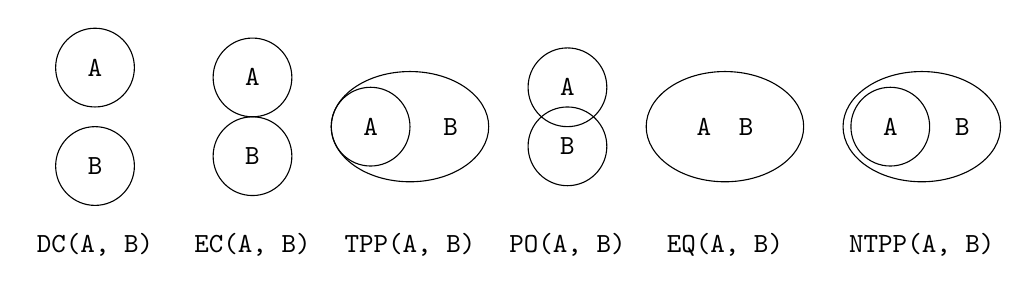
\begin{tikzpicture}
    \draw (0, 1.25) circle (0.5cm) node{\texttt{A}};
    \draw (0, 0) circle (0.5cm) node{\texttt{B}};
    \draw (0, -1) node{\texttt{DC(A, B)}};

    \draw (2, 1.125) circle (0.5cm) node{\texttt{A}};
    \draw (2, 0.125) circle (0.5cm) node{\texttt{B}};
    \draw (2, -1) node{\texttt{EC(A, B)}};

    \draw (3.5, 0.5) circle (0.5cm) node{\texttt{A}};
    \draw (4, 0.5) ellipse (1cm and 0.7cm) node[right=0.3cm]{\texttt{B}};
    \draw (4, -1) node{\texttt{TPP(A, B)}};

    \draw (6, 1) circle (0.5cm) node{\texttt{A}};
    \draw (6, 0.25) circle (0.5cm) node{\texttt{B}};
    \draw (6, -1) node{\texttt{PO(A, B)}};

    \draw (8, 0.5) ellipse (1cm and 0.7cm) node{\texttt{A} \ \ \texttt{B}};
    \draw (8, -1) node{\texttt{EQ(A, B)}};

    \draw (10.1, 0.5) circle (0.5cm) node{\texttt{A}};
    \draw (10.5, 0.5) ellipse (1cm and 0.7cm) node[right=0.3cm]{\texttt{B}};
    \draw (10.5, -1) node{\texttt{NTPP(A, B)}};

\end{tikzpicture}
    \label{fig:relations}
    \caption{Relations between regions}
\end{figure}

The problem of robot vacuum cleaning is to remove all the dirt from the floor. 
The relation that carries this information is \texttt{NTPP(dirt, Region)} where Region is the region where the dirt is actually contained.
We then decided to include another hierarchical concept to make the reasoning finer, adding the concept of a room.
Each region is then found contained within a room with the relation \texttt{NTPP(Region, Room)}.
The rooms are then connected by doors.
Doors are considered as regions that have intersection with both one room and the other (\texttt{PO(door, Room1)}, \texttt{PO(door, Room2)}) but are not contained in either.
Only the regions that are traversable by the robot are considered in this initial work without taking into account the objects in the room that are only handled by the simulation side of the framework for the time being.
The regions within a room are all close but without overlapping, thus respecting the relation \texttt{EC(Region1, Region2)}.

In order to give a proof of concept in an environment that was as verisimilar and nontrivial as possible, the study room of computer science PhD students at the University of Genoa was considered as a virtual environment.
This environment can be seen in Figure\ref{fig:environment}.
Using the representation of a real environment makes the simulation nontrivial and verisimilar.

\begin{figure}
    \centering
        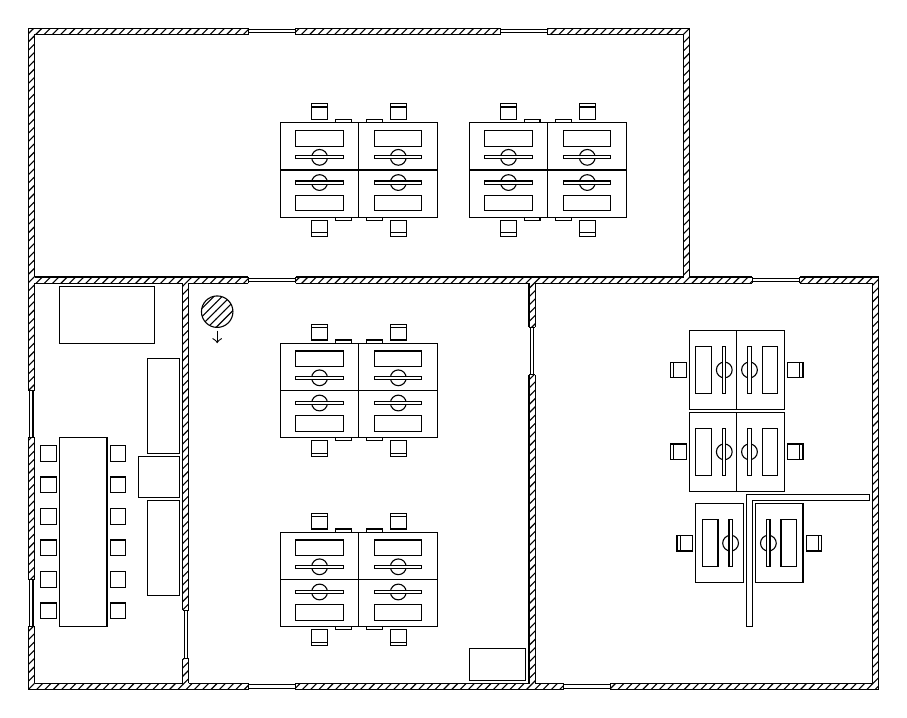
\begin{tikzpicture}[scale=0.4]
        % Area
        \draw[pattern=north east lines] (0,0) -- (0, 21) -- (21, 21) -- (21, 13.1) -- (27, 13.1) -- (27, 0) -- (0, 0);
        % Rooms
        \draw[fill=white] (0.2, 0.2) -- (0.2, 12.9) -- (4.9, 12.9) -- (4.9, 0.2) -- (0.2, 0.2);
        \draw[fill=white] (5.1, 0.2) -- (5.1, 12.9) -- (15.9, 12.9) -- (15.9, 0.2) -- (5.1, 0.2);
        \draw[fill=white] (16.1, 0.2) -- (16.1, 12.9) -- (26.8, 12.9) -- (26.8, 0.2) -- (16.1, 0.2);
        \draw[fill=white] (0.2, 13.1) -- (0.2, 20.8) -- (20.8, 20.8) -- (20.8, 13.1) -- (0.2, 13.1);

        % Door 309 Bottom
        \draw[fill=white, white] (7, 0) rectangle ++ (1.5, 0.2);
        \draw (7, 0) -- (7, 0.2) (8.5, 0) -- (8.5, 0.2);
        \draw (7, 0.05) rectangle ++ (1.5, 0.1);

        % Door 310 Bottom
        \draw[fill=white, white] (17, 0) rectangle ++ (1.5, 0.2);
        \draw (17, 0) -- (17, 0.2) (18.5, 0) -- (18.5, 0.2);
        \draw (17, 0.05) rectangle ++ (1.5, 0.1);

        % Door 309 Top
        \draw[fill=white, white] (7, 12.9) rectangle ++ (1.5, 0.2);
        \draw (7, 12.9) -- (7, 13.1) (8.5, 12.9) -- (8.5, 13.1);
        \draw (7, 12.95) rectangle ++ (1.5, 0.1);

        % Door 310 Top
        \draw[fill=white, white] (23, 12.9) rectangle ++ (1.5, 0.2);
        \draw (23, 12.9) -- (23, 13.1) (24.5, 12.9) -- (24.5, 13.1);
        \draw (23, 12.95) rectangle ++ (1.5, 0.1);

        % Door 314 Left
        \draw[fill=white, white] (7, 20.8) rectangle ++ (1.5, 0.2);
        \draw (7, 20.8) -- (7, 21) (8.5, 20.8) -- (8.5, 21);
        \draw (7, 20.85) rectangle ++ (1.5, 0.1);

        % Door 314 Right
        \draw[fill=white, white] (15, 20.8) rectangle ++ (1.5, 0.2);
        \draw (15, 20.8) -- (15, 21) (16.5, 20.8) -- (16.5, 21);
        \draw (15, 20.85) rectangle ++ (1.5, 0.1);

        % Door 308 Bottom
        \draw[fill=white, white] (0, 2) rectangle ++ (0.2, 1.5);
        \draw (0, 2) -- (0.2, 2) (0, 3.5) -- (0.2, 3.5);
        \draw (0.05, 2) rectangle ++ (0.1, 1.5);

        % Door 308-309
        \draw[fill=white, white] (4.9, 1) rectangle ++ (0.2, 1.5);
        \draw (4.9, 1) -- (5.1, 1) (4.9, 2.5) -- (5.1, 2.5);
        \draw (4.95, 1) rectangle ++ (0.1, 1.5);

        % Door 308 Top
        \draw[fill=white, white] (0, 8) rectangle ++ (0.2, 1.5);
        \draw (0, 8) -- (0.2, 8) (0, 9.5) -- (0.2, 9.5);
        \draw (0.05, 8) rectangle ++ (0.1, 1.5);

        % Door 309-310
        \draw[fill=white, white] (15.9, 10) rectangle ++ (0.2, 1.5);
        \draw (15.9, 10) -- (16.1, 10) (15.9, 11.5) -- (16.1, 11.5);
        \draw (15.95, 10) rectangle ++ (0.1, 1.5);

        % Desk Bottom Down Left
        \draw (8, 2) rectangle ++ (2.5, 1.5);
        % Chair
        \draw (9, 1.4) rectangle ++ (0.5, 0.1);
        \draw (9, 1.4) rectangle ++ (0.5, 0.5);
        \draw (9.75, 1.9) rectangle ++ (0.5, 0.1);
        % Computer
        \draw (9.25, 3.1) circle (0.25cm);
        \draw[fill=white] (8.5, 3.05) rectangle ++ (1.5, 0.1);
        \draw (8.5, 2.2) rectangle ++ (1.5, 0.5);

        % Desk Bottom Down Right
        \draw (10.5, 2) rectangle ++ (2.5, 1.5);
        % Chair
        \draw (11.5, 1.4) rectangle ++ (0.5, 0.1);
        \draw (11.5, 1.4) rectangle ++ (0.5, 0.5);
        \draw (10.75, 1.9) rectangle ++ (0.5, 0.1);
        % Computer
        \draw (11.75, 3.1) circle (0.25cm);
        \draw[fill=white] (11, 3.05) rectangle ++ (1.5, 0.1);
        \draw (11, 2.2) rectangle ++ (1.5, 0.5);

        % Desk Bottom Up Left
        \draw (8, 3.5) rectangle ++ (2.5, 1.5);
        % Chair
        \draw (9, 5.5) rectangle ++ (0.5, 0.1);
        \draw (9, 5.1) rectangle ++ (0.5, 0.5);
        \draw (9.75, 5) rectangle ++ (0.5, 0.1);
        % Computer
        \draw (9.25, 3.9) circle (0.25cm);
        \draw[fill=white] (8.5, 3.85) rectangle ++ (1.5, 0.1);
        \draw (8.5, 4.25) rectangle ++ (1.5, 0.5);

        % Desk Bottom Up Right
        \draw (10.5, 3.5) rectangle ++ (2.5, 1.5);
        % Chair
        \draw (11.5, 5.5) rectangle ++ (0.5, 0.1);
        \draw (11.5, 5.1) rectangle ++ (0.5, 0.5);
        \draw (10.75, 5) rectangle ++ (0.5, 0.1);
        % Computer
        \draw (11.75, 3.9) circle (0.25cm);
        \draw[fill=white] (11, 3.85) rectangle ++ (1.5, 0.1);
        \draw (11, 4.25) rectangle ++ (1.5, 0.5);

        \draw (8, 8) rectangle ++ (2.5, 1.5);
        \draw (9, 7.4) rectangle ++ (0.5, 0.1);
        \draw (9, 7.4) rectangle ++ (0.5, 0.5);
        \draw (9.75, 7.9) rectangle ++ (0.5, 0.1);
        % Computer
        \draw (9.25, 9.1) circle (0.25cm);
        \draw[fill=white] (8.5, 9.05) rectangle ++ (1.5, 0.1);
        \draw (8.5, 8.2) rectangle ++ (1.5, 0.5);

        \draw (10.5, 8) rectangle ++ (2.5, 1.5);
        \draw (11.5, 7.4) rectangle ++ (0.5, 0.1);
        \draw (11.5, 7.4) rectangle ++ (0.5, 0.5);
        \draw (10.75, 7.9) rectangle ++ (0.5, 0.1);

        \draw (8, 9.5) rectangle ++ (2.5, 1.5);
        \draw (9, 11.5) rectangle ++ (0.5, 0.1);
        \draw (9, 11.1) rectangle ++ (0.5, 0.5);
        \draw (9.75, 11) rectangle ++ (0.5, 0.1);
        % Computer
        \draw (9.25, 9.9) circle (0.25cm);
        \draw[fill=white] (8.5, 9.85) rectangle ++ (1.5, 0.1);
        \draw (8.5, 10.25) rectangle ++ (1.5, 0.5);

        \draw (10.5, 9.5) rectangle ++ (2.5, 1.5);
        \draw (11.5, 11.5) rectangle ++ (0.5, 0.1);
        \draw (11.5, 11.1) rectangle ++ (0.5, 0.5);
        \draw (10.75, 11) rectangle ++ (0.5, 0.1);
        % Computer
        \draw (11.75, 9.1) circle (0.25cm);
        \draw[fill=white] (11, 9.05) rectangle ++ (1.5, 0.1);
        \draw (11, 8.2) rectangle ++ (1.5, 0.5);
        % Computer
        \draw (11.75, 9.9) circle (0.25cm);
        \draw[fill=white] (11, 9.85) rectangle ++ (1.5, 0.1);
        \draw (11, 10.25) rectangle ++ (1.5, 0.5);

        \draw (14, 0.3) rectangle ++ (1.8, 1);

        \draw (1, 2) rectangle ++ (1.5, 6);
        \foreach \x in {2.25, 3.25, ..., 7.25} {
            \draw (2.6, \x) rectangle ++ (0.5, 0.5); 
            \draw (0.4, \x) rectangle ++ (0.5, 0.5); 
        }
        
        \draw (3.8, 3) rectangle ++ (1, 3);
        \draw (3.5, 6.1) rectangle ++ (1.3, 1.3);
        \draw (3.8, 7.5) rectangle ++ (1, 3);
        \draw (1, 11) rectangle ++ (3, 1.8);

        \draw (23, 2) -- (23, 6) -- (26.7, 6) -- (26.7, 6.2) -- (22.8, 6.2) -- (22.8, 2) -- (23, 2);

        \draw (21, 8.9) rectangle ++ (1.5, 2.5);
        \draw (20.4, 9.9) rectangle ++ (0.5, 0.5);
        \draw (20.4, 9.9) rectangle ++ (0.1, 0.5);
        \draw (22.1, 10.15) circle (0.25cm);
        \draw[fill=white] (22.05, 9.4) rectangle ++ (0.1, 1.5);
        \draw (21.2, 9.4) rectangle ++ (0.5, 1.5);

        \draw (22.5, 8.9) rectangle ++ (1.5, 2.5);
        \draw (24.1, 9.9) rectangle ++ (0.5, 0.5);
        \draw (24.5, 9.9) rectangle ++ (0.1, 0.5);
        \draw (22.9, 10.15) circle (0.25cm);
        \draw[fill=white] (22.85, 9.4) rectangle ++ (0.1, 1.5);
        \draw (23.3, 9.4) rectangle ++ (0.5, 1.5);

        \draw (21, 6.3) rectangle ++ (1.5, 2.5);
        \draw (20.4, 7.3) rectangle ++ (0.5, 0.5);
        \draw (20.4, 7.3) rectangle ++ (0.1, 0.5);
        \draw (22.1, 7.55) circle (0.25cm);
        \draw[fill=white] (22.05, 6.8) rectangle ++ (0.1, 1.5);
        \draw (21.2, 6.8) rectangle ++ (0.5, 1.5);

        \draw (22.5, 6.3) rectangle ++ (1.5, 2.5);
        \draw (24.1, 7.3) rectangle ++ (0.5, 0.5);
        \draw (24.5, 7.3) rectangle ++ (0.1, 0.5);
        \draw (22.9, 7.55) circle (0.25cm);
        \draw[fill=white] (22.85, 6.8) rectangle ++ (0.1, 1.5);
        \draw (23.3, 6.8) rectangle ++ (0.5, 1.5);

        \draw (21.2, 3.4) rectangle ++ (1.5, 2.5);
        \draw (20.6, 4.4) rectangle ++ (0.5, 0.5);
        \draw (20.6, 4.4) rectangle ++ (0.1, 0.5);
        \draw (22.3, 4.65) circle (0.25cm);
        \draw[fill=white] (22.25, 3.9) rectangle ++ (0.1, 1.5);
        \draw (21.4, 3.9) rectangle ++ (0.5, 1.5);

        \draw (23.1, 3.4) rectangle ++ (1.5, 2.5);
        \draw (24.7, 4.4) rectangle ++ (0.5, 0.5);
        \draw (25.1, 4.4) rectangle ++ (0.1, 0.5);
        \draw (23.5, 4.65) circle (0.25cm);
        \draw[fill=white] (23.45, 3.9) rectangle ++ (0.1, 1.5);
        \draw (23.9, 3.9) rectangle ++ (0.5, 1.5);

        % Desk Bottom Down Left
        \draw (8, 15) rectangle ++ (2.5, 1.5);
        % Chair
        \draw (9, 14.4) rectangle ++ (0.5, 0.1);
        \draw (9, 14.4) rectangle ++ (0.5, 0.5);
        \draw (9.75, 14.9) rectangle ++ (0.5, 0.1);
        % Computer
        \draw (9.25, 16.1) circle (0.25cm);
        \draw[fill=white] (8.5, 16.05) rectangle ++ (1.5, 0.1);
        \draw (8.5, 15.2) rectangle ++ (1.5, 0.5);

        % Desk Bottom Down Right
        \draw (10.5, 15) rectangle ++ (2.5, 1.5);
        % Chair
        \draw (11.5, 14.4) rectangle ++ (0.5, 0.1);
        \draw (11.5, 14.4) rectangle ++ (0.5, 0.5);
        \draw (10.75, 14.9) rectangle ++ (0.5, 0.1);
        % Computer
        \draw (11.75, 16.1) circle (0.25cm);
        \draw[fill=white] (11, 16.05) rectangle ++ (1.5, 0.1);
        \draw (11, 15.2) rectangle ++ (1.5, 0.5);

        % Desk Bottom Up Left
        \draw (8, 16.5) rectangle ++ (2.5, 1.5);
        % Chair
        \draw (9, 18.5) rectangle ++ (0.5, 0.1);
        \draw (9, 18.1) rectangle ++ (0.5, 0.5);
        \draw (9.75, 18) rectangle ++ (0.5, 0.1);
        % Computer
        \draw (9.25, 16.9) circle (0.25cm);
        \draw[fill=white] (8.5, 16.85) rectangle ++ (1.5, 0.1);
        \draw (8.5, 17.25) rectangle ++ (1.5, 0.5);

        % Desk Bottom Up Right
        \draw (10.5, 16.5) rectangle ++ (2.5, 1.5);
        % Chair
        \draw (11.5, 18.5) rectangle ++ (0.5, 0.1);
        \draw (11.5, 18.1) rectangle ++ (0.5, 0.5);
        \draw (10.75, 18) rectangle ++ (0.5, 0.1);
        % Computer
        \draw (11.75, 16.9) circle (0.25cm);
        \draw[fill=white] (11, 16.85) rectangle ++ (1.5, 0.1);
        \draw (11, 17.25) rectangle ++ (1.5, 0.5);

        % Desk Bottom Down Left
        \draw (14, 15) rectangle ++ (2.5, 1.5);
        % Chair
        \draw (15, 14.4) rectangle ++ (0.5, 0.1);
        \draw (15, 14.4) rectangle ++ (0.5, 0.5);
        \draw (15.75, 14.9) rectangle ++ (0.5, 0.1);
        % Computer
        \draw (15.25, 16.1) circle (0.25cm);
        \draw[fill=white] (14.5, 16.05) rectangle ++ (1.5, 0.1);
        \draw (14.5, 15.2) rectangle ++ (1.5, 0.5);

        % Desk Bottom Down Right
        \draw (16.5, 15) rectangle ++ (2.5, 1.5);
        % Chair
        \draw (17.5, 14.4) rectangle ++ (0.5, 0.1);
        \draw (17.5, 14.4) rectangle ++ (0.5, 0.5);
        \draw (16.75, 14.9) rectangle ++ (0.5, 0.1);
        % Computer
        \draw (17.75, 16.1) circle (0.25cm);
        \draw[fill=white] (17, 16.05) rectangle ++ (1.5, 0.1);
        \draw (17, 15.2) rectangle ++ (1.5, 0.5);

        % Desk Bottom Up Left
        \draw (14, 16.5) rectangle ++ (2.5, 1.5);
        % Chair
        \draw (15, 18.5) rectangle ++ (0.5, 0.1);
        \draw (15, 18.1) rectangle ++ (0.5, 0.5);
        \draw (15.75, 18) rectangle ++ (0.5, 0.1);
        % Computer
        \draw (15.25, 16.9) circle (0.25cm);
        \draw[fill=white] (14.5, 16.85) rectangle ++ (1.5, 0.1);
        \draw (14.5, 17.25) rectangle ++ (1.5, 0.5);

        % Desk Bottom Up Right
        \draw (16.5, 16.5) rectangle ++ (2.5, 1.5);
        % Chair
        \draw (17.5, 18.5) rectangle ++ (0.5, 0.1);
        \draw (17.5, 18.1) rectangle ++ (0.5, 0.5);
        \draw (16.75, 18) rectangle ++ (0.5, 0.1);
        % Computer
        \draw (17.75, 16.9) circle (0.25cm);
        \draw[fill=white] (17, 16.85) rectangle ++ (1.5, 0.1);
        \draw (17, 17.25) rectangle ++ (1.5, 0.5);

        \draw[black, pattern=north east lines] (6, 12) circle (0.5cm);
        \draw[->] (6, 11.4) -- (6, 11);
    \end{tikzpicture}
    \label{fig:environment}
    \caption{The test environment}
\end{figure}

The study room is divided into 4 rooms, from left to right: the common room (not considered for the current implementation), room 309, room 310 and at the top room 314.
There are workstations and cabinets in each of the rooms.
They were divided into hard-coded regions based on the location of the desks, trying to find the right balance between the whole room and excessive granularity.

Regions for the moment are only areas in the environment while they are terms for the agent. 
Obviously, the relationships between regions considered by the agent must respect what is present in the environment and vice versa, and the agent must always have an understanding of the region it is in.

\subsection{Agent: Design and Implementation}
The agent is based on the BDI paradigm and knows the entire map through RCC. 
We want to avoid in any way that the agent has Cartesian cognition of the space it is in.

The agent aims to remove all the dirt in the room and has two plans for doing so:
\begin{enumerate}
    \item \textit{clean}: removes the dirt;
    \item \textit{reach}: a plan that tells the body which region it wants to reach among those adjacent to the one it is in.
\end{enumerate}
The agent must know the logical map of the room and updates the region it is in as it goes, always keeping the term as ground as possible, the smallest region occupied by the agent.
Ultimately, the agent must be able to reason about the paths to be taken to reach its goal.
To do this requires an additional plan to be interrogated to find a sequence of noncyclic adiancent regions from the current region to the desired region.
The agent must then have a way to connect to his or her body to send requests and receive information.

The implementation was done using JaCaMo\cite{jacamo}.
As a first step, the agent creates an artifact that establishes the connection with the physical body.
The artifact then turns out to be owned by the agent, making this direct connection between agent and body without further intermediaries.
The agent then executes the \texttt{find\_and\_clean} plan, which aims to remove all the dirt in the room. 

The plan has three variants that are recursively referred to.
The first has as preconditions that there is still at least one dirt to be cleaned and that that dirt is in the same region as the agent.
In this case the agent must ask the body to reach the dirt and once it reaches it, clean it.
When it receives confirmation of the cleaning it removes that dirt from its beliefs and calls \texttt{find\_and\_clean}.
\begin{lstlisting}[language=AgentSpeak]
+!go_to_clean
    :   ntpp(Dirt, Region) & my_region(Region) & dirt(Dirt)
    <-  gain(Dirt);
        .wait({+gained});
        clean(Dirt);
        .wait({+cleaned});
        -ntpp(Dirt, Region);
        !go_to_clean.
\end{lstlisting}
The second, on the other hand, only predicts that there is still dirt.
If the agent uses this plan, it is because the dirt is not in the same region and therefore must move to the region where the dirt is contained.
To do this, the agent has another plan \texttt{move\_to} that allows it to reach the region where the dirt is.
\begin{lstlisting}[language=AgentSpeak]
+!go_to_clean
    :   ntpp(Dirt, Region) & dirt(Dirt)
    <-  !move_to(Region);
        !go_to_clean.
\end{lstlisting}
The \texttt{move\_to} plan also has variations.
In particular, it must take into account the room in which it is located; if in fact the region sought is in another room, the agent must look for a door that will take him into it, reach it, and then once inside it find the path to the region in which the dirt is located or another door if necessary.
If, on the other hand, he is in the same room, he must find and follow the sequence of regions that lead him to the desired one.
The \texttt{move\_to} plan, in addition to finding the path is also concerned with following it, that is, waiting until a message has arrived for each region from the body indicating that it has been reached before moving on to consider the next one with the \texttt{follow\_path} plan.
\begin{lstlisting}[language=AgentSpeak]
+!move_to(region)
    :   my_region(CurrentRegion) & 
        not sameroom(CurrentRegion, Region) & 
        ntpp(Region, Room) & ec(Door, Room)
    <-  ?find_path(CurrentRegion, Door, Path);
        .reverse(Path, ReversePath);
        !follow_path(ReversePath);
        !move_to(Region).

+!move_to(Region)
    :   my_region(CurrentRegion)
    <-  ?find_path(CurrentRegion, Region, Path);
        .reverse(Path, ReversePath);
        !follow_path(ReversePath).
\end{lstlisting}
For the time being, no path search optimization logic is implemented but simply the agent searches for one that is walkable.

Finally, the agent has a \texttt{clean} plan that allows it to remove dirt by communicating to its body to perform the action.
This plan is called when the agent is on dirt and is the one that eliminates it.
It has no preconditions, because indeed a robot vacuum cleaner can vacuum even where it is already clean, it is the \texttt{find\_and\_clean} plan that calls it at the right time.

Finally, communication with Godot is implemented within the Java artifact that implements a Websocket client and can send two types of messages:
\begin{itemize}
    \item \lstinline|{"type": "gain", "target": Target}|: sent to reach a Target region;
    \item \lstinline|{"type": "clean", "target": Target}|: sent to clean the Target dirt.
\end{itemize}

\subsection{Environment: Design and Implementation}
The environment must represent the map presented in Figure\ref{fig:environment} with the due physical characteristics of the objects and walls and must handle agent displacement and dirt removal.
The regions must be inserted into the scene in a physical way: the robot must not reason about them, it must find path and realize it has reached the region, so they must be something the robot can virtually interact with.
Note that regions also need to be inserted at doors that make it possible to pass from one room to another.

The environment was implemented with Godot.
Godot is an open-source game development software that allows to place objects within a 3D virtual environment and attach scripts to some objects.
The environment was built as visible in Figure\ref{fig:godot} respecting the features shown in Figure\ref{fig:environment}.
Regions have been implemented in this version as \texttt{Marker3D}s and thus as individual points near which the agent must pass.
The robot is implemented as \texttt{CharacterBody3D} and has attached a script that implements agent connection, movement, and dirt removal.

\begin{figure}
    \centering
    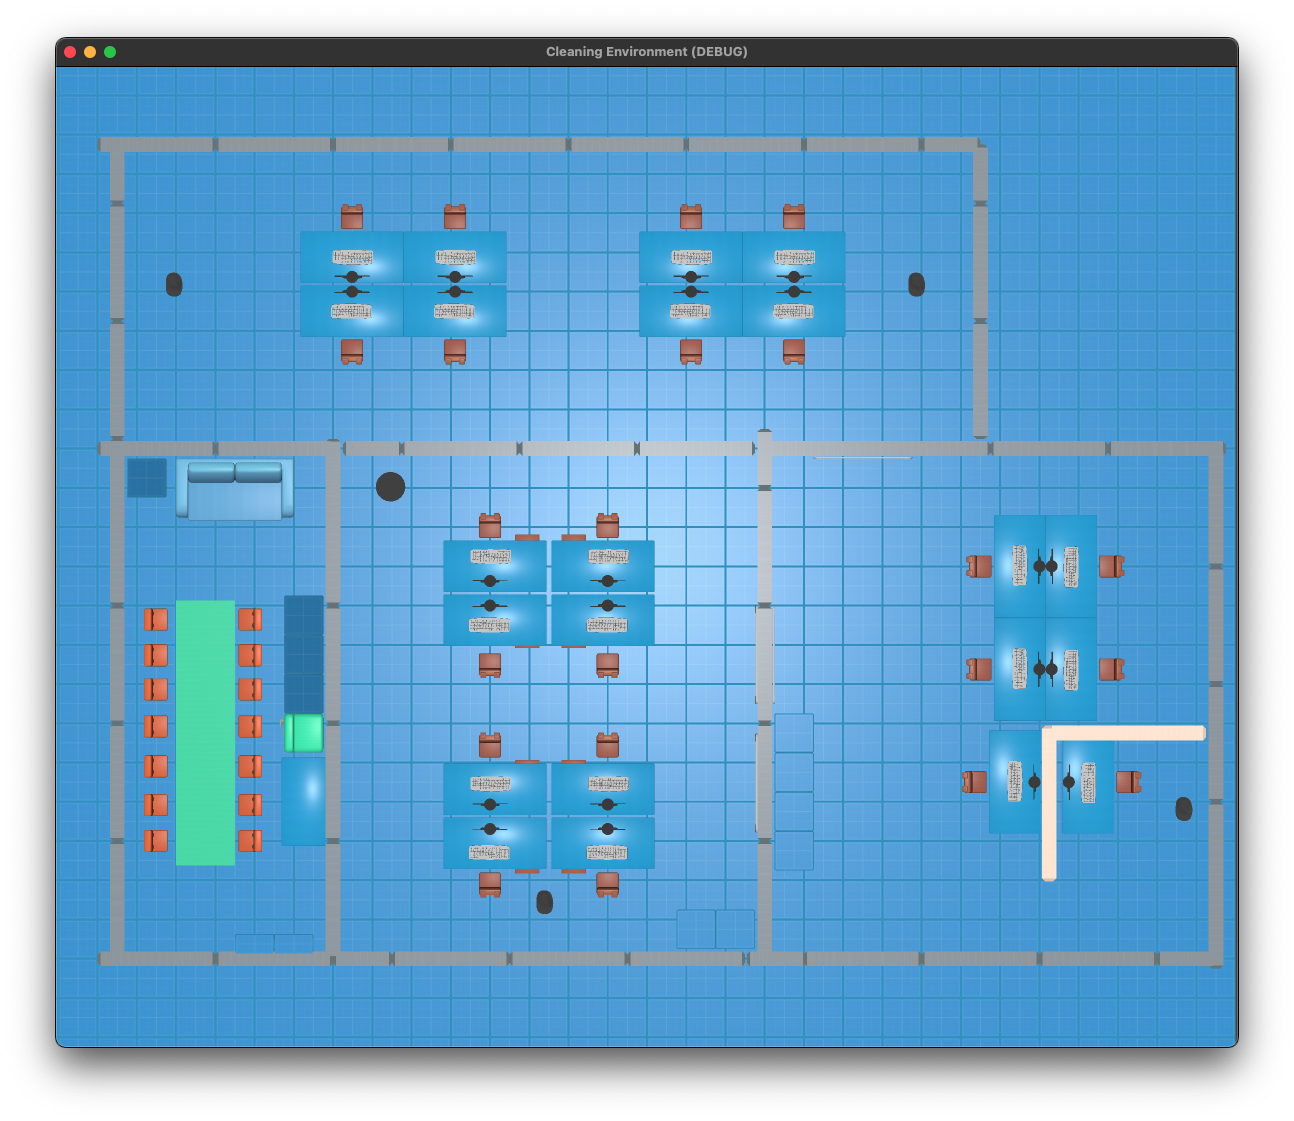
\includegraphics[width=0.75\textwidth]{sections/imgs/env.png}
    \label{fig:godot}
    \caption{The Godot environment}
\end{figure}

The \texttt{NavigationRegion3D} node was used to implement path finding. This type of node creates a map of walkable surfaces from the nodes it has as children.
In our case the entire environment except the vacuum cleaner itself is instantiated as a child of this node, making everything walkable.
The robot is then implemented using the \texttt{CharacterBody3D} node as its main with a \texttt{NavigationAgent3D} as its child that implements the robot's walk on the map given by the NavigationRegion3D.
The algorithm that is used by the \texttt{NavigationAgent3D} to find the best path is a version of A$^\star$ on the continuum with steps of unfixed length.

%\begin{figure}
%    \centering
%    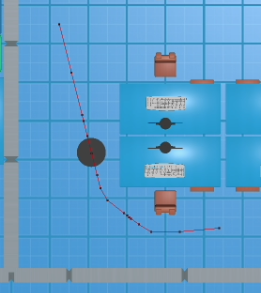
\includegraphics[scale=0.4]{sections/imgs/trajectory.png}
%    \label{fig:trajectory}
%    \caption{The followed trajectory}
%\end{figure}

The connection is implemented as a WebSocket Server directly within the script so again the robot communicates directly with its agent.
This creates a 1-to-1 agent-robot correlation that may be useless for the moment but is game changing as we move from a single agent to having multiple agents and multiple robots in the same environment.

When the agent sends a message to the robot of type \texttt{\{"type": "gain", "target": "regionX"\}} the received region is entered as the target of NavigatAgent3D.
It then calculates the shortestPath to reach it and follows it step by step. The robot's degrees of rotation are not constrained in any way, nor is the length of the space it travels at each step.
When it has reached the goal it sends a message \texttt{\{"type": "inform", "code": "gained"\}} to the agent informing it that it is ready to perform the next task, be it moving to another region or cleaning up.
If the agent requests cleaning then the node depicting dirt from the robot is destroyed and a message \texttt{\{"type": "inform", "code": "cleaned"\}} is sent to the agent awaiting new instructions.

	\section{Results}
	\label{sec:results}
In this section we briefly present the results obtained.
The agent communicates correctly with the virtual robot and manages to complete its task completely.
It is possible to see the operation of the framework in two videos, \href{https://youtu.be/dQbiNx36fNs}{one} in which the agent simply performs its task and \href{https://youtu.be/iuQfDgS0oUE}{one} in which the debug mode is activated in which we can see the paths calculated by the robot.

\begin{figure}
    \centering
    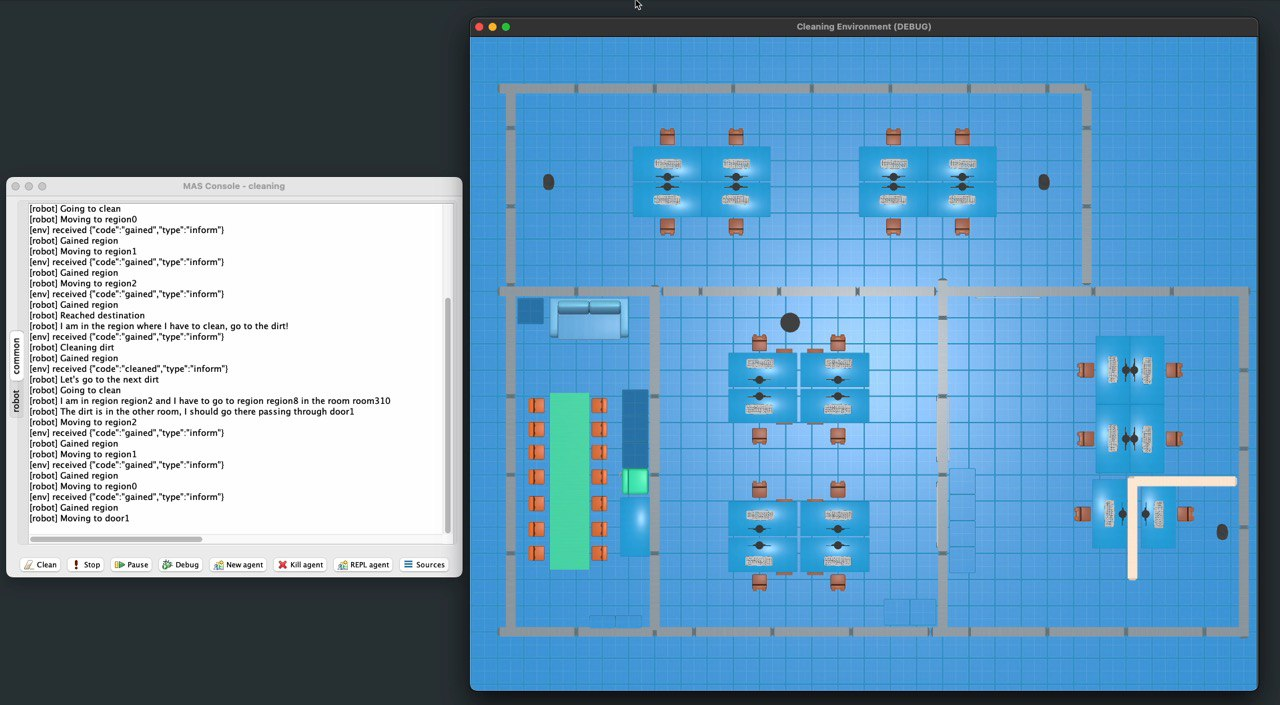
\includegraphics[width=\textwidth]{sections/imgs/screen.jpeg}
    \caption{The agent in action.}
    \label{fig:screen}
\end{figure}
In the Figure\ref{fig:screen} you can see the framework in action.
On the left is the JaCaMo window in which the agent is implemented while on the right is visible Godot and the robot you want in the room.

In the implementation we were able to completely separate the logical reasoning part from the coordinate management part.
For the time being, however, the agent is still not looking for the best path but simply for a walkable path from one region to another.
The results confirm that the robot in this way has full freedom of rotation by producing non-regular paths and that the ability to find paths in the instrument continuum is enhanced.
The robot's path planning, in addition to the features already listed, also has the ability to adapt to any occlusions dynamically, recalculating the path in case something has moved without having to take it into account logically.

This implementation is easily scalable from both the environment and multi-agent system perspectives.
In fact, the region-based logic model makes it very easy to expand the environment both in width and depth (increasing its accuracy); in fact, we have already demonstrated the operation of subregions by implementing rooms.
The connection between agent and robot implemented end-to-end with a private artifact of the agent and a proven script of the robot also makes the multi-agent system scalable without the need for further major modifications.

	\section{Conclusions and Future Work}
	We presented a framework in which a BDI agent controls a robot vacuum cleaner with a precise division of responsibilities, giving logical task management to the agent and physical management of movement and cleaning to the robot.
Going through the key theoretical concepts, we showed how the environment must be studied and designed for this kind of approach, then going on to see the actual implementation of all components with JaCaMo and Godot.
The implementation aims not to discretize the robot's movements by forcing them within some predetermined logical actions but by choosing the actions logically, implementing them in the continuum.

The current implementation has many limitations, the two most important being the management of regions on the virtual environment side and the insertion of objects into the logical map.
In Godot, the region should be implemented as an Area3D, looking for the nearest location without having to reach the center or a specific point.
Agent side, the map should also contain objects and objects should be considered, thinking of a scenario where they are most meaningful.

Future work will therefore go in these directions.
In addition to this, an exploratory version of the framework will be implemented in which the agent faces the challenge of cleaning without knowing the map and without knowing where the dirty areas are.
The real challenge in this version will be to figure out how to subdivide the walkable regions, what are the criteria that make a region stand on its own or not.

  \bibliographystyle{unsrt}
  \bibliography{bibliography}

\end{document}